% Created 2020-09-11 Fri 10:04
% Intended LaTeX compiler: pdflatex
\documentclass[unicode, 12pt, xdvipdfmx, aspectratio=43]{beamer}
\usepackage[utf8]{inputenc}
\usepackage[T1]{fontenc}
\usepackage{graphicx}
\usepackage{grffile}
\usepackage{longtable}
\usepackage{wrapfig}
\usepackage{rotating}
\usepackage[normalem]{ulem}
\usepackage{amsmath}
\usepackage{textcomp}
\usepackage{amssymb}
\usepackage{capt-of}
\usepackage{hyperref}
\usepackage[backend=bibtex, style=authoryear, maxcitenames=2]{biblatex}
\addbibresource{../resources/anthology.bib}
\addbibresource{../resources/my.bib}
\let\oldcite\cite
\renewcommand{\cite}[1]{{\scriptsize\reffont{(\oldcite{#1})}}}
\newcommand{\citet}[2][\footnotesize]{{\reffont#1\citeauthor*{#2} (\citeyear{#2})}}
\newcommand{\mycite}[1]{{\scriptsize\reffont({\citeauthor*{#1}, \citeyear{#1}})}}
\newcommand{\myfootcite}[1]{\footnote{\tiny\reffont\citetitle{#1}, \citeauthor*{#1}, \citeyear{#1}.}}
\usepackage{url}
\usetheme[numbering=fraction]{metropolis}
\setbeamertemplate{items}[default]
\setbeamertemplate{itemize item}{\small\raise0.5pt\hbox{$\blacksquare$}}
\setbeamertemplate{itemize subitem}{\footnotesize\raise1.5pt\hbox{$\bullet$}}
\setbeamertemplate{itemize subsubitem}{\scriptsize\raise1.5pt\hbox{$\blacktriangleright$}}
\setbeamertemplate{enumerate item}{\textbf{(\arabic{enumi})}}
\addtolength{\skip\footins}{6pc plus 10pt}
\usepackage{xltxtra}
\usepackage{booktabs}
\usepackage[absolute,overlay]{textpos}
\usepackage{pgfpages}
\usefonttheme{professionalfonts}
\usepackage[T1]{fontenc}
\usepackage{fontspec}
\XeTeXlinebreaklocale "ja"
\usepackage{xeCJK}
\setsansfont[BoldFont={Fira Sans Bold}]{Fira Sans Book}
\setCJKmainfont{Noto Sans CJK JP}
\setCJKsansfont{Noto Sans CJK JP}
\setCJKromanfont{Noto Serif CJK JP}
\xeCJKDeclareCharClass{CJK}{`※}
\newfontfamily\firasans{Fira Sans}
\newfontfamily\emojifont{Noto Emoji}
\newfontfamily\octicons{github-octicons}
\newfontfamily\materials{Material Icons}
\newfontfamily\reffont{Times New Roman}
\renewcommand{\baselinestretch}{1.3}
\usetheme{default}
\author{出口 ~ 祥之 \\ \lower2.0pt\hbox{\materials} \texttt{deguchi@ai.cs.ehime-u.ac.jp}}
\date{2020/09/11 ~ 第 2 回 NLG/MT Reading Group}
\title{Dynamic Programming Encoding for Subword Segmentation in Neural Machine Translation}
\subtitle{(He et al., ACL 2020)}
\institute{}
\hypersetup{
 pdfauthor={出口 ~ 祥之 \\ \lower2.0pt\hbox{\materials} \texttt{deguchi@ai.cs.ehime-u.ac.jp}},
 pdftitle={Dynamic Programming Encoding for Subword Segmentation in Neural Machine Translation},
 pdfkeywords={},
 pdfsubject={},
 pdfcreator={Emacs 27.1 (Org mode 9.3.7)}, 
 pdflang={English}}
\begin{document}

\maketitle

\begin{frame}[label={sec:orge400b88}]{\hbox{\octicons} Links}
\begin{block}{\raise0.5pt\hbox{\octicons} Paper}
\begin{block}{\url{https://www.aclweb.org/anthology/2020.acl-main.275/}}
\end{block}
\end{block}
\begin{block}{\raise0.5pt\hbox{\octicons} Source Code}
\begin{block}{\url{https://github.com/xlhex/dpe}}
\end{block}
\end{block}
\end{frame}

\begin{frame}[label={sec:org7734d15}]{Introduction}
\vspace{-0.2cm}
\begin{block}{動的計画法を用いた新たなサブワード分割法を提案}
\vspace{-0.2cm}
\small
\begin{itemize}
\item 目的言語文の分割を潜在変数と見做し,周辺化 \vspace{-0.2cm}
\item ``\alert{Mixed character-subword Transformer}'': \\ 原言語文が与えられたときの目的言語文の分割を獲得
\end{itemize}
\end{block}
\begin{block}{}
\vspace{-1.0cm}
\metroset{block=fill}
\begin{block}{NMT におけるサブワード分割}
\vspace{-0.4cm}
\small
\begin{center}
\begin{tabular}{rl}
\textbf{貪欲法:} & バイトペア符号化 (BPE)\myfootcite{sennrich-etal-2016-neural}, WordPiece\myfootcite{schuster-nakajima-2012-japanese}\\
\textbf{確率的アルゴリズム:} & ユニグラムLM\myfootcite{kudo-2018-subword}, BPE-dropout\myfootcite{provilkov-etal-2020-bpe}\\
\textbf{動的計画法:} & 本論文の提案手法 \vspace{-0.3cm}\\
\end{tabular}
\end{center}
\end{block}
\end{block}

\vspace{0.3cm}
\end{frame}

\begin{frame}[label={sec:org615a2a6}]{Related Work (Greedy Segmentation)}
\begin{block}{BPE \cite{sennrich-etal-2016-neural}, WordPiece \cite{schuster-nakajima-2012-japanese}}
\begin{itemize}
\item 隣接する頻出サブワードから順に,予め指定した \\ 語彙数に到達するまで再帰的に結合 (BPE)
\item 語彙数とデコード速度はトレードオフ
\begin{itemize}
\item (語彙数を小さくするだけであれば文字単位でよい)
\item テキスト圧縮の技術を利用
\item 語彙数の上限を制約とし,文長が短くなるような \\ 分割を得るアルゴリズム
\end{itemize}

\item[{例:}] \textrm{unconscious → un + conscious}
\end{itemize}
\end{block}
\end{frame}

\begin{frame}[label={sec:org5098f82}]{Related Work (Stochastic Segmentation)}
\begin{block}{ユニグラムLM \cite{kudo-2018-subword}, BPE-dropout \cite{provilkov-etal-2020-bpe}}
\begin{itemize}
\item \normalsize 複数分割候補を得られる
\begin{itemize}
\item ユニグラムLM: 尤度ベースでサンプリング
\item BPE-dropout: BPE 結合時に確率的に棄却
\item NMT 訓練時に分割を確率的に得ることでデータ拡張 \textrm{(Data Augumentation)} \sffamily の効果
\begin{itemize}
\item モデルの頑健性向上
\end{itemize}
\end{itemize}

\item[{例:}] \textrm{unconscious → \{un + concious, uncon + scious\}}
\end{itemize}
\end{block}
\end{frame}


\begin{frame}[label={sec:org2692db4}]{\normalsize Related Work (Dynamic Programming Algorithms)}
\small
\begin{block}{音声認識 \cite{wang-etal-2017-sequence}}
\begin{itemize}
\item 取り得る全ての分割や入出力間のアライメントの確率を動的計画法により計算
\end{itemize}
\end{block}

\begin{block}{非自己回帰 NMT モデル \cite{chan-etal-2020-imputer, saharia-etal-2020-nonautoregressive}}
\begin{itemize}
\item \textbf{Imputer} \cite{chan-etal-2020-imputer} : \\ Connectionist Temporal Classification (CTC) を用い,定数回のデコードで出力とその順序を予測
\item 非自己回帰 NMT モデルに Imputer を適用 \cite{saharia-etal-2020-nonautoregressive}
\end{itemize}
\end{block}
\end{frame}

\section{Proposed Method}
\label{sec:org8c348fe}
\begin{frame}[label={sec:orgf4662e8}]{Latent Subword Segmentation - Definitions}
\begin{block}{\hspace{-0.75cm}目的言語文の分割を潜在変数とみなす}
\begin{columns}
\begin{column}{1.0\columnwidth}
\begin{itemize}
\item \(M\) 個のサブワード: \(\{\boldsymbol{y}_{z_i, z_{i+1}}\}_{i=1}^M\)
\begin{itemize}
\item \(\boldsymbol{y} = (y_1, \ldots, y_T)\): 目的言語文の文字列
\item \(\boldsymbol{z} = (z_1 ,\ldots, z_{M+1})\): 境界位置系列
\begin{itemize}
\item \(0 = z_1 < z_2 < \ldots < z_M < z_{M+1} = T\) (昇順)
\end{itemize}
\item \(\boldsymbol{y}_{a,b}\): \((a+1)^\text{th}\) から \(b^\text{th}\) まで結合したサブワード
\end{itemize}
\end{itemize}
\end{column}

\begin{column}{0.42\columnwidth}
\begin{textblock*}{\linewidth}(230pt, 40pt)
    \centering
    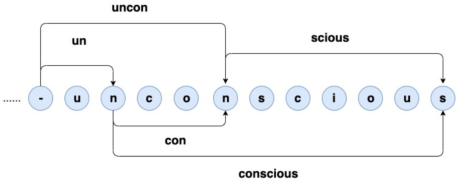
\includegraphics[width=\linewidth]{./figure/Figure1.pdf}
\end{textblock*}
\end{column}
\end{columns}
\end{block}

\begin{columns}
\begin{column}{0.5\columnwidth}
\begin{block}{例:}
\footnotesize
\begin{itemize}
\item 辞書 \(\mathcal{V} = \{\text{c, a, t, ca, at}\}\)
\item 目的言語文 \(\boldsymbol{y} = \text{cat}\)
\end{itemize}
\end{block}
\end{column}

\begin{column}{0.5\columnwidth}
\footnotesize

\begin{center}
\begin{tabular}{ll}
\toprule
\(\boldsymbol{z}\) & サブワード列\\
\midrule
\((0,1,3)\) & (c, at)\\
\((0,2,3)\) & (ca, t)\\
\((0,1,2,3)\) & (c, a, t)\\
\bottomrule
\end{tabular}
\end{center}
\end{column}
\end{columns}
\end{frame}

\begin{frame}[label={sec:org164a588}]{Latent Subword Segmentation - Likelihood}
\begin{block}{連鎖律を用いてサブワード列の対数尤度を表現}
\begin{itemize}
\item 各サブワード位置において語彙の確率分布を生成
\begin{equation*}
  \log p(\boldsymbol{y},\boldsymbol{z} | \boldsymbol{x}) = \sum_{i=1}^{|\boldsymbol{z}|} \log p(\boldsymbol{y}_{z_i, z_{i+1}} | \boldsymbol{y}_{z_1, z_2},\ldots,\boldsymbol{y}_{z_{i-1}, z_i}, \boldsymbol{x})
\end{equation*}
※ \(\boldsymbol{x}\) : 原言語文
\item 殆どの NMT では \(\boldsymbol{z}\) を暗黙的に \(\log p(\boldsymbol{y}, \boldsymbol{z}) \approx \log p(\boldsymbol{y})\) と仮定
\end{itemize}
\end{block}
\end{frame}

\begin{frame}[label={sec:org5330b8a}]{\normalsize Latent Subword Segmentation - Latent Variable}
\begin{block}{\(\boldsymbol{z} \in \mathcal{Z}_{y} (\boldsymbol{y} \text{の分割集合})\) を潜在表現とみなす}
\begin{itemize}
\item \(p(\boldsymbol{y} | \boldsymbol{x}) = \sum_{\boldsymbol{z}} p(\boldsymbol{y}, \boldsymbol{z} | \boldsymbol{x})\) とする
\begin{equation*}
  \small \log p(\boldsymbol{y} | \boldsymbol{x}) = \log\sum_{\boldsymbol{z}\in\mathcal{Z}_y}\exp\sum_{i=1}^{|\boldsymbol{z}|} \log p(\boldsymbol{y}_{z_i, z_{i+1}} | \boldsymbol{y}_{z_1, z_2},\ldots,\boldsymbol{y}_{z_{i-1}, z_i}, \boldsymbol{x})
\end{equation*}
※ 対数周辺尤度の下限: \(\log p(\boldsymbol{y} | \boldsymbol{x}) \ge \log p(\boldsymbol{y}, \boldsymbol{z} | \boldsymbol{x})\)

\item 各サブワードの確率が条件部のコンテキストの分割に依存するため,巨大な空間 \(\mathcal{Z}_y\) 上での厳密な周辺化は組み合わせ爆発を起こす
\begin{itemize}
\item コンテキストが次に来るサブワードの確率に \\ 影響しないモデルが必要
\end{itemize}
\end{itemize}
\end{block}
\end{frame}

\begin{frame}[label={sec:org11020e8}]{A Mixed Character-Subword Transformer}
\begin{block}{文字に基づいてサブワードを生成する Transformer}
\begin{itemize}
\item 条件部のコンテキストを文字のみに
\begin{equation*}
  \log p(\boldsymbol{y}, \boldsymbol{z} | \boldsymbol{x}) = \sum_{i=1}^{|\boldsymbol{z}|} \log p(\boldsymbol{y}_{z_i, z_{i+1}} | y_{z_1}, \ldots, y_{z_i}, \boldsymbol{x})
\end{equation*}

\item \(\boldsymbol{y}\) の各文字位置 \(t\) において,次に来るサブワード \(w \in \mathcal{V}\) の分布を以下に基づいて生成
\begin{equation*}
  p(w | y_{1}, \ldots, y_{t}, \boldsymbol{x}) = \frac{\exp(f(y_1,\ldots,y_t)^\top e(w))}{\sum_{w' \in \mathcal{V}}\exp(f(y_1,\ldots,y_t)^\top e(w'))}
\end{equation*}
\begin{itemize}
\item \vspace{-0.5cm} \(f(\cdot)\) : Transformer により条件部の計算
\item \(e(\cdot)\) : ソフトマックス層の重み
\end{itemize}
\end{itemize}
\end{block}
\end{frame}

\begin{frame}[label={sec:org8e01be5}]{A Mixed Character-Subword Transformer}
\begin{columns}
\begin{column}{0.65\columnwidth}
\begin{block}{\(t\) ステップ目のモデル出力}
\begin{enumerate}
\item \(t\) ステップ目でサブワード \(w\) を生成
\item サブワード \(w\) の文字をデコーダに入力 ( \(t+1\) から \(t+|w|\) まで )
\item \(t+|w|\) ステップ目で次のサブワードを生成
\end{enumerate}
\end{block}
\end{column}

\begin{column}{0.35\columnwidth}
\begin{center}
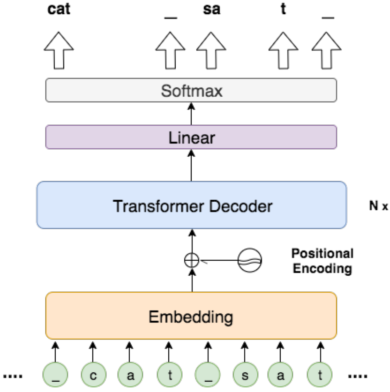
\includegraphics[width=1.1\linewidth]{./figure/Figure2.pdf}
\end{center}
\end{column}
\end{columns}
\end{frame}

\begin{frame}[label={sec:org38d0a8f}]{Optimization}
\begin{block}{目的関数 \(\mathcal{L}(\theta)\) を最大化}
\begin{equation*}
  \mathcal{L}(\theta) = \sum_{(\boldsymbol{x}, \boldsymbol{y}) \in \mathcal{D}} \log P_\theta (\boldsymbol{y} | \boldsymbol{x})
\end{equation*}
\end{block}

\begin{block}{必要な計算}
\begin{itemize}
\item 周辺尤度の計算
\item 対数周辺尤度の勾配計算
\end{itemize}
\end{block}
\end{frame}

\begin{frame}[label={sec:orgf1f277c}]{Exact Marginalization}
\begin{block}{動的計画法を用いて周辺尤度を計算}
\begin{itemize}
\item サブワードの出力確率が文字のみによって得られるため動的計画法によって対数周辺尤度が計算可能
\end{itemize}
\vspace{-0.5cm}

\begin{center}
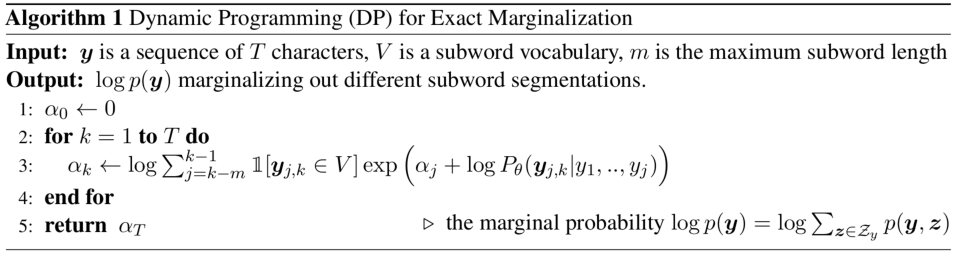
\includegraphics[width=1.05\linewidth]{./figure/Algorithm1.pdf}
\end{center}
\vspace{-0.5cm}
\begin{itemize}
\item 計算量:  \(\mathcal{O}(mT)\)
\begin{itemize}
\item \(m\) : 語彙に含まれる最長の単語の文字数
\end{itemize}
\end{itemize}
\end{block}
\end{frame}

\begin{frame}[label={sec:org029c38a}]{Gradient Computation}
\begin{block}{計算量に関する問題点}
\begin{itemize}
\item 通常の Transformer デコーダより 8 倍遅く,メモリ使用量も増加 \footnote{\texttt{PyTorch}での著者実装で比較}
\begin{itemize}
\item DP アルゴリズムと文字レベルでの演算による系列長の増加が原因
\end{itemize}
\end{itemize}
\end{block}

\begin{block}{対処法}
\begin{itemize}
\item Transformer のレイヤ数を 6 から 4 に削減
\item 16 ステップ分勾配蓄積 \textrm{(Gradient Accumulation)} してからパラメタ更新
\end{itemize}
\vspace{0.5cm}
\end{block}
\end{frame}

\begin{frame}[label={sec:orgb5d62a1}]{Segmenting Target Sentences}
\begin{block}{Dynamic Programming Encoding (DPE): \\ 最大事後確率を持つ目的言語文の分割を探索}
\begin{center}
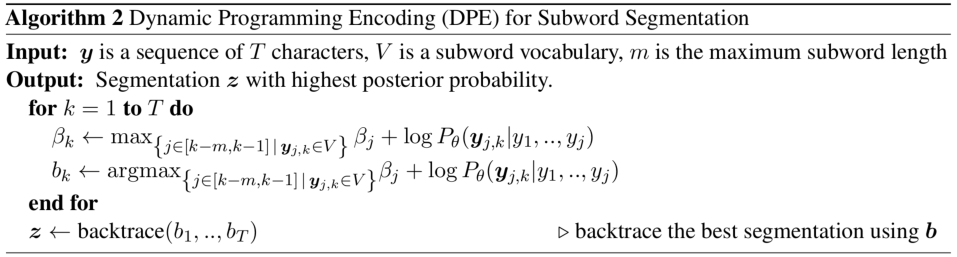
\includegraphics[width=\linewidth]{./figure/Algorithm2.pdf}
\end{center}
\end{block}
\end{frame}

\begin{frame}[label={sec:org4cab1f0}]{Segmenting Target Sentences}
\begin{itemize}
\item Mixed character-subword Transformer は \\ \alert{訓練データ}の\alert{目的言語文}の分割のためのみに使用
\item 分割した文で通常のサブワード Transformer を訓練
\end{itemize}
\begin{center}
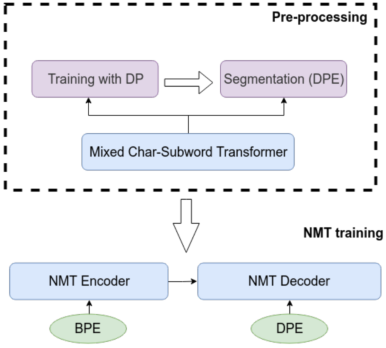
\includegraphics[width=0.5\linewidth]{./figure/Figure3.pdf}
\end{center}
\end{frame}

\begin{frame}[label={sec:orgf40ec73}]{Experiments}
\begin{description}
\item[{データセット}] WMT09 En-Hu, WMT14 En-De, WMT15 En-Fi, WMT16 En-Ro, WMT18 En-Et
\item[{モデル}] 
\end{description}
\begin{center}
\begin{tabular}{ll}
\toprule
NMT アーキテクチャ & Transformer base\\
分割 (原言語側) & BPE-dropout \((p=0.05)\)\\
   (目的言語側) & DPE (提案手法)\\
\bottomrule
\end{tabular}
\end{center}
\end{frame}

\begin{frame}[label={sec:org6e5143b}]{Main Results}
\begin{center}
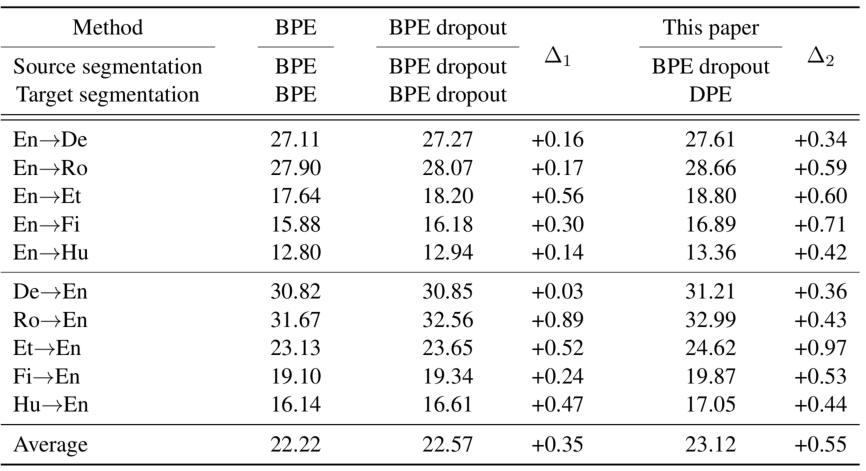
\includegraphics[width=1.05\linewidth]{./figure/Table2.pdf}
\end{center}
\end{frame}

\begin{frame}[label={sec:orge8f1f67}]{Segmentation Examples}
\begin{center}
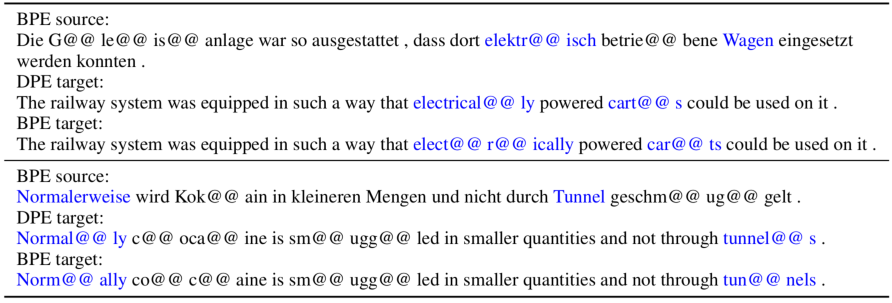
\includegraphics[width=1.05\linewidth]{./figure/Table3.pdf}
\end{center}
\begin{itemize}
\item 他の例は論文参照
\end{itemize}
\end{frame}

\begin{frame}[label={sec:orgb3df2c5}]{Conditional Subword Segmentation}
\begin{block}{原言語文を条件部に入れず,LM で分割}
\vspace{-0.3cm}
\begin{center}
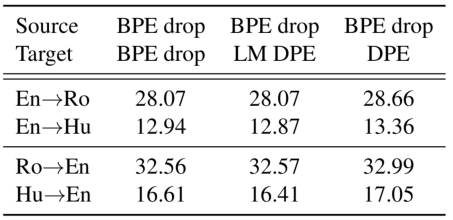
\includegraphics[width=0.5\linewidth]{./figure/Table5.pdf}
\end{center}

\vspace{-0.5cm}
\end{block}
\begin{block}{同一の目的言語文で原言語側を変えて違いを比較}
\vspace{-0.3cm}
\begin{center}
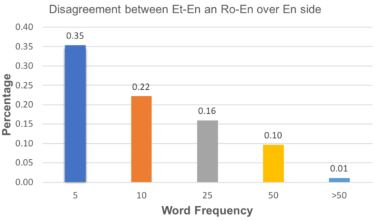
\includegraphics[width=0.5\linewidth]{./figure/Figure4.pdf}
\end{center}
\end{block}
\end{frame}

\begin{frame}[label={sec:orgcaf11ad}]{Conditional Subword Segmentation}
\begin{block}{\small 原言語文が BPE-dropout によって変化することの有効性}
\begin{center}
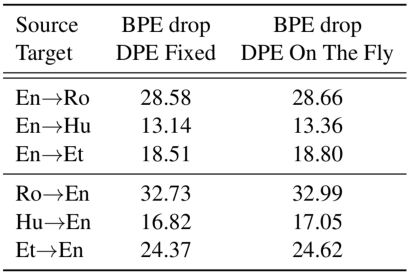
\includegraphics[width=0.6\linewidth]{./figure/Table6.pdf}
\end{center}
\end{block}
\end{frame}

\begin{frame}[label={sec:org98c0f27}]{DPE vs BPE}
\begin{block}{目的言語側の分割アルゴリズムを変えて比較}
\begin{center}
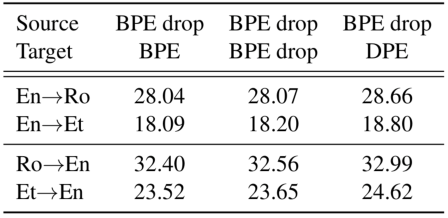
\includegraphics[width=0.6\linewidth]{./figure/Table7.pdf}
\end{center}
\end{block}
\end{frame}

\begin{frame}[label={sec:org1cef520}]{Conclusion}
\begin{block}{新たなサブワード分割法 \\ Dynamic Programming Encoding を提案}
\begin{itemize}
\item \alert{Mixed character-subword Transformer} により \\ 目的言語文を分割
\begin{itemize}
\item 目的言語文の分割を潜在変数と見做して周辺化
\item 条件部のコンテキストを文字にすることで \\ 動的計画法が適用可能に
\item 分割時は事後確率が最大となる分割を出力
\end{itemize}
\end{itemize}
\begin{itemize}
\item BPE だけでなく BPE-dropout と比較しても \\ 翻訳性能が向上
\end{itemize}
\end{block}
\end{frame}
\end{document}